\section{\large From bass/treble to an equalizer}
%For each problem, outline the problem in your own words, your approach, what you did and why you did it.
The task is to implement a tunable FIR equalizer with five equally spaced (linear scale) bands.
Using the frequency domain equivalence method the FIR filter coefficients can be determined by defining the magnitude response, transforming to the time-domain, windowing and translating to obtain a causal response. A function that constructs the filter coefficients was implemented where filter order and window type are parameters. The code is shown in Figure~\ref{fig:equalizer5band}.
\begin{figure}[H]
\center
\begin{lstlisting}
function [h] = equalizer5band(G1, G2, G3, G4, G5, n, W);
%INPUT: Band gains: G1, G2, G3, G4, G5. Approximate length: n. Window: W.
%OUTPUT: Impulse response/FIR filter coefficients: h.
m = round(n/10);
H = [G1*ones(1, m) , G2*ones(1, m) , G3*ones(1, m) , G4*ones(1, m) , ...
     G5*ones(1, m) , G5*ones(1, m) , G4*ones(1, m) , G3*ones(1, m) , ...
     G2*ones(1, m) , G1*ones(1, m)];
h = ifftshift(ifft(H, 'symmetric'));
L = length(h);
if W == 0 %rectangualr window (technically unnecessary code)
   h = h; %do nothing
elseif W == 1
   h = h.*hanning(L)';
elseif W == 2
   h =h.*hamming(L)'; 
end
end %eof
\end{lstlisting}
\caption{The \texttt{equalizer5band} function used to generate the FIR filter coefficients.}
\label{fig:equalizer5band}
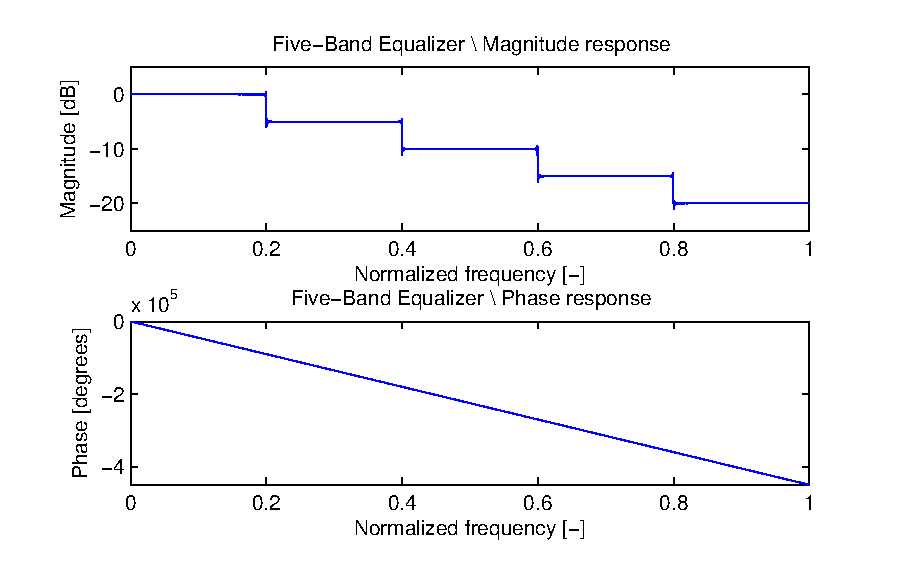
\includegraphics[scale=1]{./picture/FiveBandEqualizer.eps}%
\caption{Magnitude and phase response of the transfer function of a five-band FIR equalizer with band gains decreasing in steps of 5 dB from the lowest to the highest normalized frequency. Ringing at the edges is caused by the use of a rectangular window in this case. See Figure~\ref{fig:equalizer5band}. The filter order in this case is 4999 (IR length 5000).}
\label{fig:FiveBandEqualizer}
\end{figure}

\newpage
\begin{figure}[H]
\center
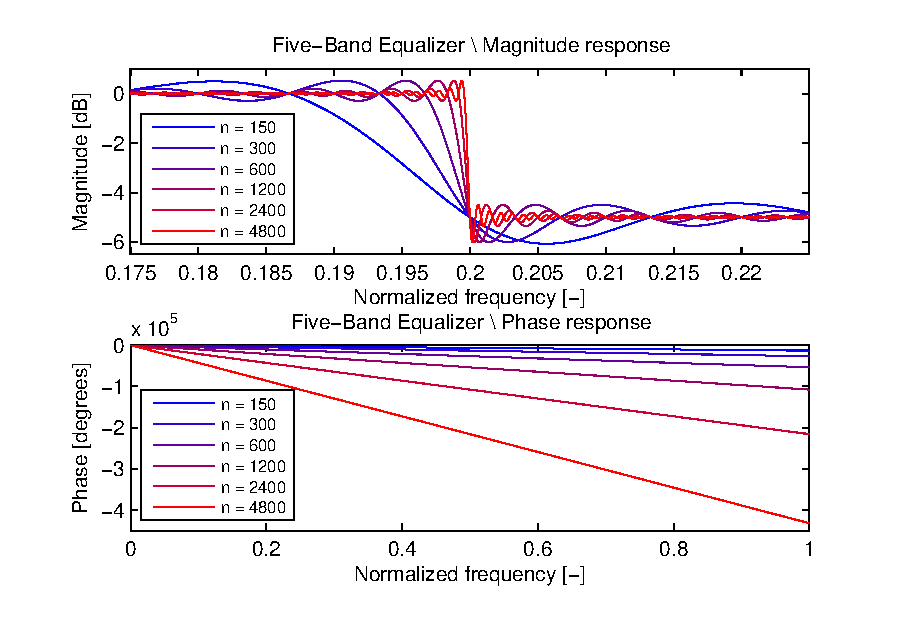
\includegraphics[scale=1]{EqualizerOrderRectangle.eps}%
\caption{Equalizer frequency response (rectangular window function) for several IR lengths $n$. Ringing caused by the discontinuous rectangular window is clear and increases with the order. The phase response is linear, since the filter type is FIR and had zero-phase before translation.}
\label{fig:EqualizerOrderRectangle}
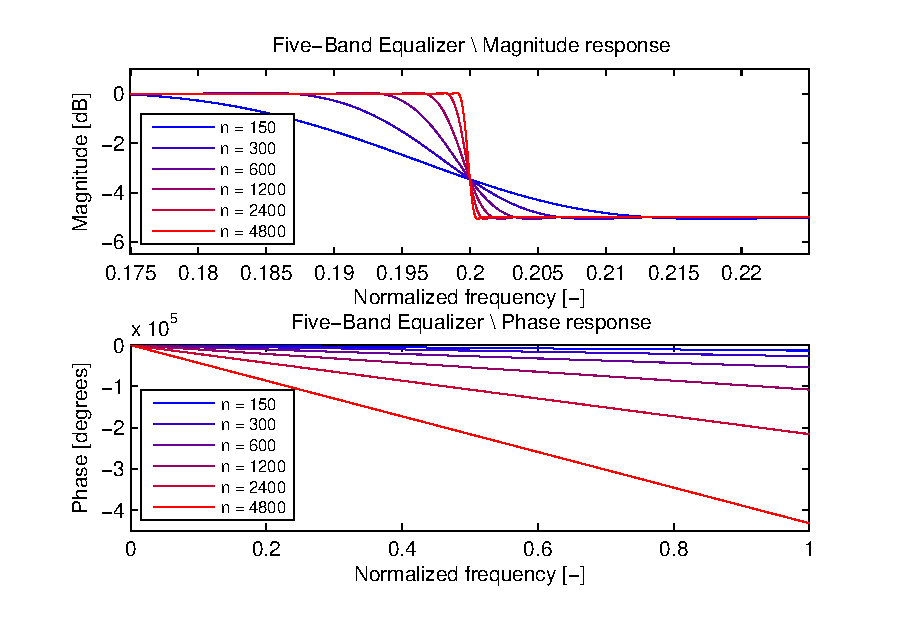
\includegraphics[scale=1]{./picture/EqualizerOrderHanning.eps}%
\caption{Equalizer frequency response (using Hann window function) for several IR lengths $n$. Compare with Figure~\ref{fig:EqualizerOrderRectangle} to see the clear improvement in smoothness of the magnitude response. Note also that the slope of the phase response is proportional to the IR length (also Figure~\ref{fig:EqualizerOrderRectangle}). This is also as expected since a time translation by $\tau$ corresponds to a phase shift proportional to $\tau$.}
\label{fig:EqualizerOrderHanning}
\end{figure}

\newpage
%Choose the order of the filter yourself and explain your choice.
\noindent Higher order results in a greater phase slope and therefore more initial delay (besides the cost), but the approximation is much better. The relations between order, phase and approximation are illustrated in Figure~\ref{fig:EqualizerOrderRectangle} (rectangular window function) and Figure~\ref{fig:EqualizerOrderHanning} (Hann window function). A filter order of 499 (corresponding to IR length $n=500$) may be chosen for practical purposes (e.g. equalizing music), since an order of this size gives a somehat reasonable approximation without too many samples (less processing time, less memory usage and less delay as benefits). The magnitude response in Figure~\ref{fig:EqualizerOrderHanning} show that this choice is middle ground.\\

%Zero-pad your impulse response to twice/ten times the length and plot again the frequency response.
%Explain what you see.
\noindent Zero-padding the IR increases samples in the time domain and hence in the frequency domain. The spectral resolution increases with the number of samples. By comparing the resulting plots this effect was observed in the magnitude response (but not in the phase response however). Choosing a smoother window gives a less pronounced effect (since there is less ringing). \\

%Pass a white noise signal through your filter and plot the spectra of the original and the filtered signal on top of each other.
\noindent The result of processing white noise using the equalizer settings in Figure~\ref{fig:FiveBandEqualizer} is shown in Figure~\ref{fig:EqualizedNoise}. As expected, a stepwise descent corresponding to the magnitude response can be clearly seen.
\begin{figure}[H]
\center
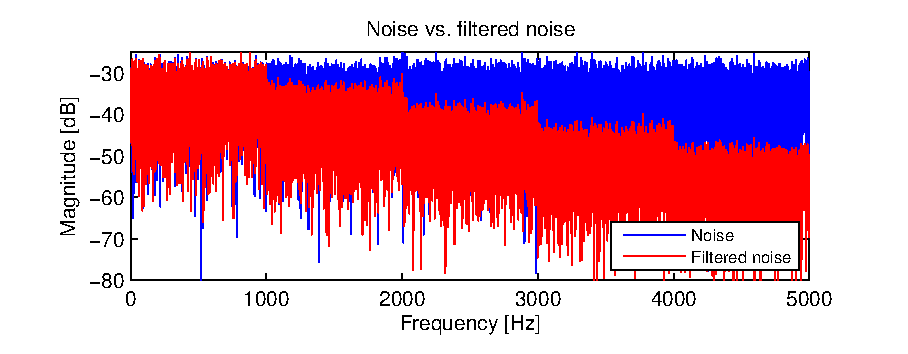
\includegraphics[scale=1]{./picture/EqualizedNoise.eps}%
\caption{White noise signal filtered using the frequency response from Figure~\ref{fig:FiveBandEqualizer} (order 4999). The expected descent by 5 dB for each step is clearly visible in the output spectrum.}
\label{fig:EqualizedNoise}
\end{figure}

%Process your favourite piece of music through the filter and listen to it! It's fantastic, isn't it? No.
\noindent The result of processing \texttt{piano.wav} using the equalizer settings in Figure~\ref{fig:FiveBandEqualizer} is shown in Figure~\ref{fig:EqualizedPiano}. A stepwise descent is no longer clear, but attenuation appears to increase steadily with frequency.
\begin{figure}[H]
\center
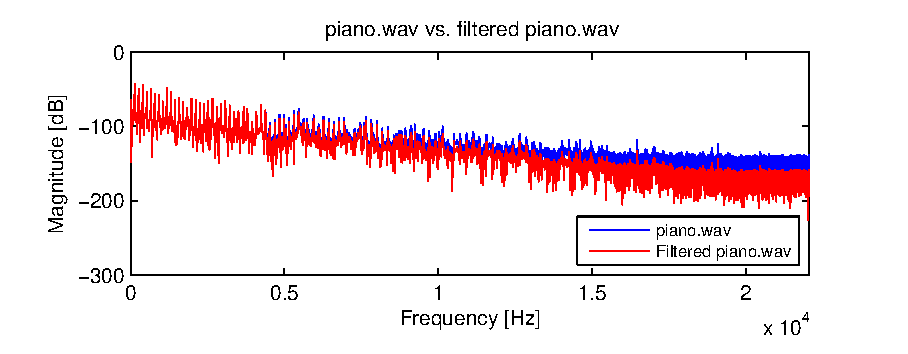
\includegraphics[scale=1]{./picture/EqualizedPiano.eps}%
\caption{Sound \texttt{piano.wav} filtered using the frequency response from Figure~\ref{fig:FiveBandEqualizer} (order 4999). Attenuation increases steadily in accordance with the magnitude response of the applied filter.}
\label{fig:EqualizedPiano}
\end{figure}
